The initial step of our work is the study of the existing MC TBR model and its
behaviour. Following the examination of its features (simulation parameters), we
present efficient means of evaluating this model on large sets of points in HPC
environment, preprocessing techniques designed to adapt collected datasets for
surrogate modelling, and our attempts at feature space reduction to achieve the
lowest possible number of dimensions.


\subsection{Expensive Model Description}
\label{sec:expensive-model-description}

The MC TBR model that we understand to be the expensive function for our
surrogate modelling is fundamentally a Monte Carlo simulation based on the OpenMC
framework. At input the software expects a set of 19~parameters, discrete and
continuous, that are fully listed in~\cref{tbl:params}. Following a brief period of
time (usually on the order of tens of seconds), during which a fixed number of events is simulated, the software outputs the
mean and the standard deviation of the TBR aggregated over the simulated run. The
former of these two outputs we accept to be the output TBR value that is subject
to approximation.

\begin{table}[h]
	\centering
	{\footnotesize
		\begin{tabular}{llll}
		\toprule
		Parameter name & Type & Domain & Description\\
		\midrule
		TODO & TODO & TODO & TODO\\
		\bottomrule
		\end{tabular}
	}
	\caption{Input parameters supplied to the MC TBR simulation.}
	\label{tbl:params}
\end{table}

In our work, we often reference TBR points or samples. These are simply vectors
in the feature space generated by Cartesian product of domains of all
features---parameters from~\cref{tbl:params}.

Since most surrogate models
that we employ assume overall continuous inputs, we take steps to unify our
feature interface in order to attain this property. In particular, we eliminate
discrete features by embedding each such feature into a finite multitude of
continuous features using standard one-hot encoding. This option is available to
us since discrete domains that generate our feature space are finite in
cardinality and relatively small in size. And while it renders all features continuous, the
modification comes at the expense of increasing the dimensionality of the
feature space, which is comprised of 27 features from this point on.


\subsection{Dataset Generation}
\label{sec:dataset-generation}

TODO
\begin{enumerate}
	\item grid search vs random sampling
	\item from a set of sampled points to evaluated TBR values
	\item tech deployed at Hypatia: dockerised sampler \& dataframe-driven querying
	\item run 0, 1, 2 parameters
\end{enumerate}


\subsection{Preprocessing}
\label{sec:preprocessing}

TODO
\begin{enumerate}
	\item discrete feature embedding
	\item standardisation
\end{enumerate}


\subsection{Dimensionality Reduction}
\label{sec:dimred}

Model training over high-dimensional parameter spaces may be facilitated by carefully reducing the number of variables used to describe the space. For many applications, feature selection strategies succeed in identifying a sufficiently representative subset of the original input variables; however, all given variables were assumed to be physically relevant to the MC TBR model. Feature extraction methods, on the other hand, aim to identify a transformation from the parameter space which decreases dimensionality; even if no individual parameter is separable from the space, some linear combinations of parameters or nonlinear functions of parameters may be.

\begin{figure}[h]
  \centering
    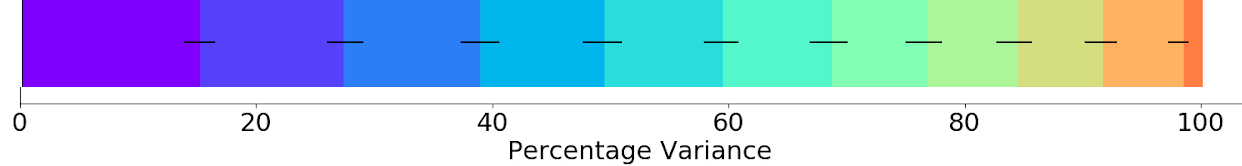
\includegraphics[width=0.6\linewidth]{fig2_pca.jpg}
    \caption{Cumulative variance for optimal features identified by PCA}
  \label{fig:pca}
\end{figure}

\begin{wrapfigure}{r}{0.5\textwidth}
  \vspace{-55pt}
  \begin{center}
    \hspace*{-.3\columnsep}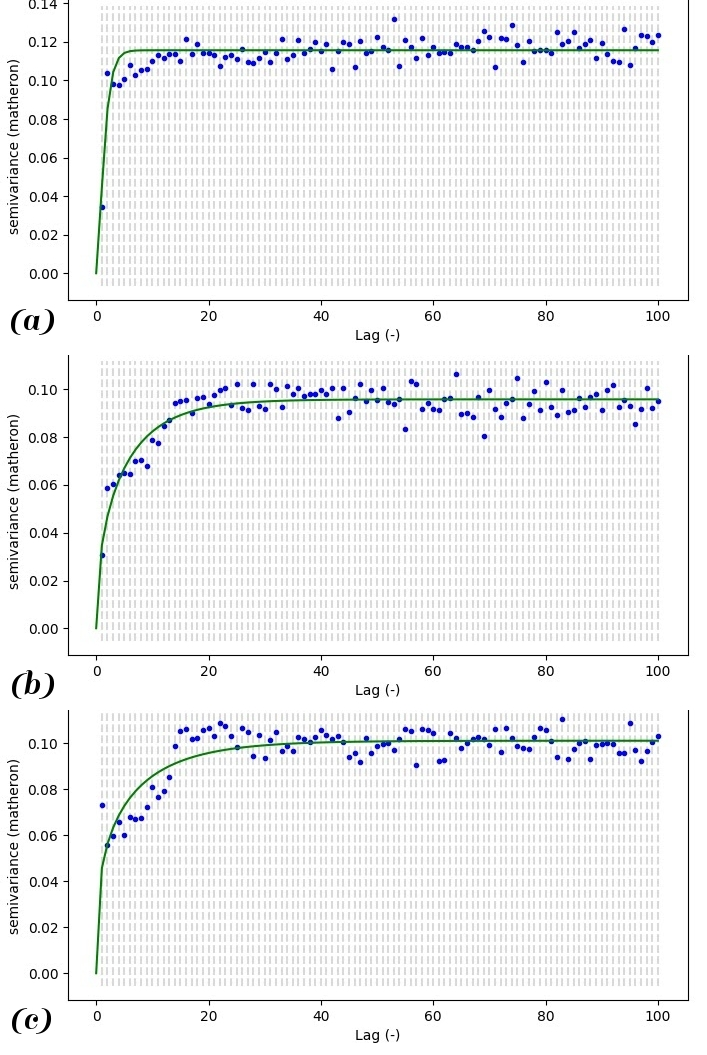
\includegraphics[width=0.58\textwidth]{fig3_allvar.jpg}
    \caption{Semivariograms for MC TBR data with coolant materials: (a) $He$, (b) $H_2O$, (c) $D_2O$}
    \label{fig:var}
  \end{center}
  \vspace{-110pt}
\end{wrapfigure}

\subsubsection{Principal Component Analysis}

To pursue linear feature extraction, principal component analysis (PCA) was performed via scikit-learn on a set of 300,000 uniform samples of the MC TBR model. 

Figure \ref{fig:pca} shows the resultant cumulative variance of the feature vectors identified by PCA. The similar share of variance among all eleven features demonstrated irreducibility of the TBR model by linear methods.

\subsubsection{Variogram Computations}

Kriging, or Gaussian process regression, is a geostatistical surrogate modelling technique which relies on correlation functions over distance (lag) in the paramater space [2]. Although kriging performed poorly for our use case due to high dimensionality, these correlation measures gave insight into similarities between discrete-parameter slices of the data.

Figure \ref{fig:var} shows the Matheron semivariance [3] for three discrete slices with coolant material varied, but all other discrete parameters fixed. Fits [4] to the Matérn covariance model confirmed numerically that the coolant material is the discrete parameter with the greatest distinguishability in the MC TBR model. 


** TODO: Make sure discrete slices are mentioned before this **

\subsubsection{Autoencoders}

TODO: Question: is it accurate to say this represents nonlinear feature extraction? re my intro paragraph

TODO
\begin{enumerate}
	\item working principle
	\item application on single slice
	\item application on mixed slice data
\end{enumerate}


